\documentclass[a4paper, 11pt, nofonts, 
twoside, sfsidenotes, nobib, justified]{tufte-handout}

\makeatletter
% Paragraph indentation and separation for normal text
\renewcommand{\@tufte@reset@par}{%
	\setlength{\RaggedRightParindent}{1.0pc}%
	\setlength{\JustifyingParindent}{1.0pc}%
	\setlength{\parindent}{1pc}%
	\setlength{\parskip}{0pt}%
}
\@tufte@reset@par

% Paragraph indentation and separation for marginal text
\renewcommand{\@tufte@margin@par}{%
	\setlength{\RaggedRightParindent}{0.5pc}%
	\setlength{\JustifyingParindent}{0.5pc}%
	\setlength{\parindent}{0.5pc}%
	\setlength{\parskip}{0pt}%
}
\makeatother

\usepackage[backend = biber, style = alphabetic]{biblatex}
\addbibresource{quellen.bib}

\DefineBibliographyStrings{german}{andothers={et\addabbrvspace al\adddot}}

%\usepackage{natbib}
%\bibliographystyle{unsrtnat}

\usepackage{mdframed}
\mdfdefinestyle{sonstiges}{
	%backgroundcolor=lightgray,
	linecolor=lightgray!50!black,
	linewidth=2pt,
	bottomline = false,
	topline=false,
	rightline=false,
	frametitlefont={\bfseries},
	frametitle = {}
	%leftline=false
}
\mdfdefinestyle{wichtig}{
	backgroundcolor=lightgray,
	linecolor=lightgray!50!black,
	linewidth=2pt,
	bottomline = false,
	topline=false,
	rightline=false,
	frametitlefont={\bfseries}
	%leftline=false
}

\usepackage[ngerman]{babel}
\usepackage[utf8]{inputenc}
\usepackage[T1]{fontenc}

\usepackage{amsmath, amssymb, amsthm, amsfonts}
\usepackage{pgfplots, tikz, graphics}
\usepackage{mdframed, listings, xcolor, hyperref, url}

\usepackage{caption, newfloat, lipsum}
\captionsetup{labelfont = bf, figurename = Abb.}

\geometry{top = 2.5cm, bottom = 1.5cm, left = 1.5cm, rmargin = 7cm}

\newmdenv[
linecolor=lightgray,
backgroundcolor=white,
bottomline =false,
topline = false,
rightline = false,
linewidth = 2pt
]{grau_balken}

\definecolor{codegreen}{rgb}{0,0.6,0}
\definecolor{codegray}{rgb}{0.5,0.5,0.5}
\definecolor{codepurple}{rgb}{0.58,0,0.82}
\definecolor{backcolour}{rgb}{0.95,0.95,0.92}

\lstdefinestyle{bunt}{
	%backgroundcolor=\color{backcolour},   
	commentstyle=\color{codegreen},
	numberstyle=\footnotesize\sffamily\color{codegray},
	stringstyle=\color{codepurple},
	basicstyle=\ttfamily \footnotesize,
	breakatwhitespace=false,         
	breaklines=true,                 
	captionpos=t,                    
	keepspaces=true,                 
	numbers=left,
	%	float = [htb],                    
	numbersep=5pt,                  
	showspaces=false,                
	showstringspaces=false,
	showtabs=false,                  
	tabsize=2,
	frame=top,frame=bottom,  
	keywordstyle = \bfseries, 
	keywordstyle =\color{blue!50!black} \bfseries,
}
\lstdefinestyle{bw}{
	%backgroundcolor=\color{backcolour},   
	%commentstyle=\color{codegreen},
	numberstyle=\footnotesize\sffamily\color{codegray},
	%stringstyle=\color{codepurple},
	breakatwhitespace=false,         
	breaklines=true,                 
	captionpos=t,                    
	keepspaces=true,                 
	numbers=left,
	%float = [htb],                    
	numbersep=5pt,                  
	showspaces=false,                
	showstringspaces=false,
	showtabs=false,                  
	tabsize=2,
	frame=top,frame=bottom,  
	keywordstyle = \bfseries, 
	%keywordstyle =\color{blue!50!black} \bfseries,
}
\lstset{literate=%
	{Ö}{{\"O}}1
	{Ä}{{\"A}}1
	{Ü}{{\"U}}1
	{ß}{{\ss}}1
	{ü}{{\"u}}1
	{ä}{{\"a}}1
	{ö}{{\"o}}1
}
%\DeclareFloatingEnvironment[placement=h!, name=Code]{listing}
\renewcommand{\lstlistingname}{Code}\DeclareCaptionFormat{listing}{\rule{\dimexpr\textwidth\relax}{0.4pt}\par\vskip1pt#1#2#3}
\captionsetup[lstlisting]{format=listing,singlelinecheck=false, margin=0pt, labelsep=space,labelfont=bf}

\usepackage{titlesec, siunitx}
\setcounter{secnumdepth}{2}
\titleformat{\section}{\bfseries\LARGE}{\S\thesection}{.5cm}{}

\usepackage{enumitem}
\setlist[enumerate,1]{leftmargin = *, noitemsep}

%\usepackage{roboto, roboto-mono}
%\usepackage[bb=fourier]{mathalpha}

\usepackage{fancyhdr}
\pagestyle{fancy}

\definecolor{bsg1}{RGB}{43,46,131}
\definecolor{bsg2}{RGB}{0,145,158}
\definecolor{bsg3}{RGB}{119,174,88}

\newcommand{\bsgrule}{{\color{bsg1}\rule{.33\linewidth}{2pt}}{\color{bsg2}\rule{.33\linewidth}{2pt}}{\color{bsg3}\rule{.33\linewidth}{2pt}}}
%}

\usepackage{titlesec, lastpage, qrcode}
\titleformat{\section}{\bfseries\large}{\thesection~|}{.5em}{}

\makeatletter
% Paragraph indentation and separation for normal text
\renewcommand{\@tufte@reset@par}{%
\setlength{\RaggedRightParindent}{0pc}%
\setlength{\JustifyingParindent}{0pc}%
\setlength{\parindent}{0pc}%
\setlength{\parskip}{0pt}%
}
\@tufte@reset@par

% Paragraph indentation and separation for marginal text
\renewcommand{\@tufte@margin@par}{%
\setlength{\RaggedRightParindent}{0pc}%
\setlength{\JustifyingParindent}{0pc}%
\setlength{\parindent}{0pc}%
\setlength{\parskip}{0pt}%
}
\makeatother

\lhead{Lukas Semrau}
\rhead{\small\thepage}
\usepackage{cmbright, subcaption, colortbl, tabularx}
\sisetup{locale = DE}  
\sisetup{
per-mode=fraction,
fraction-function=\tfrac 
}
%\usepackage{mathptmx}
\usepackage{multirow}
\begin{document}
\begin{marginfigure}
	\centering
	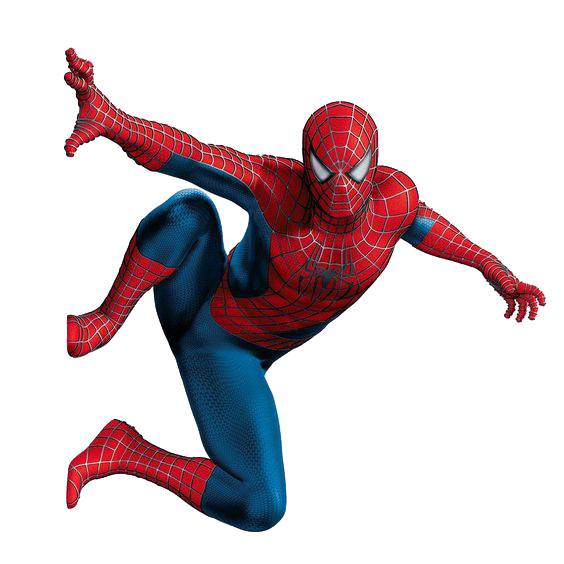
\includegraphics[width = \linewidth]{material/08 deko2.png}
\end{marginfigure}
{\bfseries{\LARGE Stoppt er die U-Bahn?} }
\vspace{1em}

In der vorliegenden Szene stoppt Spiderman durch seine Spinnennetze einen Zug, um diesen vor dem Absturz zu bewahren. Beim Betrachten der Szene stellen sich folgende Fragen:
\begin{enumerate}
	\item Sind die Fäden in der Lage, den Zug aufzuhalten?
	\item Ist Spiderman stark genug, um diese Seile zu halten, ohne dass seine Arme herausgerissen werden?
\end{enumerate}
\section{Halten die Fäden die Bremsung aus?} 
\subsection{Der Zug}
Bei dem Zug handelt es sich um das \textsc{2200-series} Modell aus Chicago mit einer Kapazität von 46 Sitzplätzen und einer Masse von $m_\text{Wagon}=\SI{21500}{\kilogram}$. \cite{WSem03} Geht man davon aus, dass auf jeden Sitzplatz zwei Stehplätze kommen, und der Zug zu 85\% ausgelastet ist, sind in einem Wagon 
$$n = 85\%\cdot \left( 46 + 2\cdot 46 \right)=117,4\approx 117.$$ In einem Frame kann man ablesen, dass der Zug aus 6 solcher Wagons besteht. Insgesamt sind in dem Zug also $n_\text{ges.} = 6\cdot n \approx 700$ zu rettende Personen. Nach \cite{WSem04} wiegt der durchschnittliche US-Amerikaner $m_\text{Person}=\SI{82.6}{\kilogram}$. Die gesamtmasse des Zuges beträgt also
\begin{align*}
	m = n_\text{ges.} \cdot m_\text{Person} + 6\cdot m_\text{Wagon}=\SI{190740}{\kilogram}.
\end{align*}
\subsection{Der Bremsvorgang}
In einem Frame sieht man, dass der Zug eine Ausgangsgeschwindigkeit von 80 Meilen pro Stunde hat. Dies entspricht ca. $v_0=\SI{35}{\meter\per\second}$. \cite{WSem02} Misst man die Zeit zwischen dem zweiten Versuch, den Zug mittels den Spinnenfäden zu stoppen ($v_E=\SI{0}{\meter\per\second}$), und dem Stillstand, so erhält man das Ergebnis $t=\SI{45}{\second}$. Mit den Formeln $a=\frac{\Delta v}{\Delta t}$ und $F = m\cdot a$ kann man nun die Kraft zum Bremsen\footnote{Diese Kraft ist negativ, weil die Kraft entgegen der Bewegungsrichtung wirkt. Im folgenden rechne ich aus Gründen der Einfachheit mit dem positiven Wert weiter.} bestimmen.
\begin{align*}
	F_\text{Brems} = m \cdot \frac{\Delta v}{\Delta t} = m \cdot \frac{v_E -v_0}{\Delta t} = \SI{-151588.3}{\newton}
\end{align*}
\subsection{Die Fäden}
Die Frage, die nun noch offen ist, ist, ob die Fäden diese Kraft aushalten können. Nach \cite{WSem07} ist diese Kraft 
\begin{align}
	F_n=\sigma \cdot A,
\end{align}
\begin{marginfigure}
	\centering
	\includegraphics[width = \linewidth]{material/02 fäden.png}
	\caption{Frame, in dem man die Fäden abzählen kann.}
	\label{fig1}
\end{marginfigure}
wobei $\sigma$ die Zugfestigkeit des Materials ist. (bei Spinnenseide: $\sigma = \SI{1.1e9}{\pascal}$, \cite{WSem08}). $A$ ist die Querschnittsfläche des Materials. Angenommen die Fäden seien Zylinder, mit der Grundfläche $G=\pi\cdot (\frac d2)^2$, so kann man zählen, dass Spiderman 16 dieser Fäden spinnt, die Querschnittfläche beträgt also 
\begin{align}
	A=16G=16\cdot \pi\cdot \left(\frac d2\right)^2
\end{align}
\newpage
\begin{marginfigure}
	\centering
	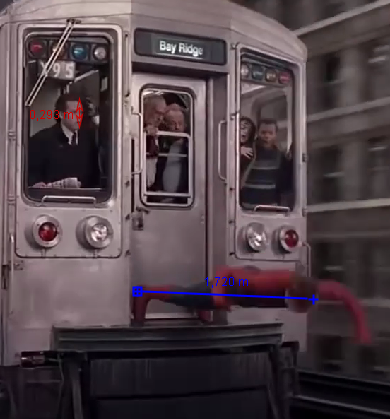
\includegraphics[height = 4.5cm]{material/05 gersicht.png}
	\caption{}
	\label{fig2:a}
\end{marginfigure}
\begin{marginfigure}
	\centering
	\vspace{.5cm}
	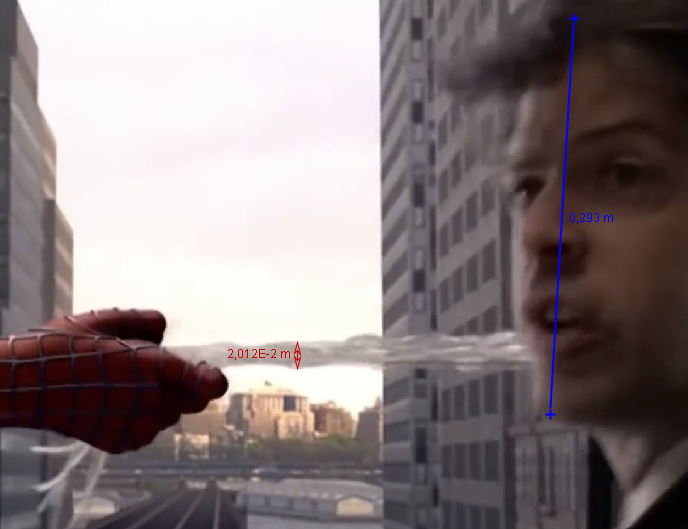
\includegraphics[height =4cm]{material/06 faden neu.png}
	\caption{}
	\label{fig2:b}
\end{marginfigure}
Damit man die Querschnittsfläche und damit auch die Kraft bestimmen kann, muss man den Durchmesser eines Fadens bestimmen: Über Abb. \ref{fig2:a} kann man gut mit Hilfe der Größe des Schauspielers Tobey Maguire \cite{WSem11} die Länge des Gesichts des Komparsen im Hintergrund bestimmen. In einem anderen Frame (Abb. \ref{fig2:b}) kann man über diese Gesichtsgröße den Durchmesser $d_\text{ges}=\SI{0.02}{\meter}$ eines Fadenbündels (rechts von Spiderman). In Abb. \ref{fig1} kann man sehen dass diese Fadenbündel aus 8 Fäden bestimmen. Ein Faden hat also den Durchmesser $d=\SI{0.0025}{\meter}$. \\
Die Kraft, die diese Fäden halten können ist also
\begin{align*}
	F_n=\sigma \cdot A = \sigma \cdot 16 \cdot \pi \cdot \left(\frac d2\right)^2 &= \SI{1.1e9}{\pascal} \cdot 16\cdot \pi \cdot\left(\frac{\SI{0.0025}{\meter}}{2}\right)^2\\&=\SI{86393.8}{\newton} 
\end{align*}
\begin{mdframed}[style = wichtig, frametitle = {Fazit}]
	Die Kraft, die die Fäden maximal aufbringen können, ist gerade einmal $\frac{F_n}{F_\text{Brems}}=0,57\%$ der benötigten Kraft. Mit den verwendeten Werte ist diese Rettungsaktion also \underline{nicht} möglich.
\end{mdframed}
\section{Ist Spiderman stark genug?}
Die Frage die sich letztlich noch stellt ist, ob Spiderman die Kraft aushalten würde, die von den Fäden ausgeht. In dem Marvel-Wiki \cite{WSem10} heißt es:
\begin{quote} 
	Spider-Man besitzt übermenschliche Stärke, welche es ihm erlaubt etwa 20 Tonnen zu heben.\footnote{Natürlich ist ein ``Marvel-Wiki'' nicht die vertrauenswürdigste Quelle, allerdings handelt es sich über einen Superhelden mit übernatürlichen Kräften, zu dem es keine Studien geben wird.}
\end{quote}
Er hat also die Kraft $F_\text{Spiderman}=\SI{20e3}{\kilogram}\cdot 9.81=\SI{196200}{\newton}$.
\begin{mdframed}[style = wichtig, frametitle = Fazit]
	Angenommen die Fäden könnten den Zug aufhalten, so wäre Spiderman auch in der Lage diese Kraft zu halten, und den Zug somit zu stoppen.
\end{mdframed}
%\bibliography{quellen.bib}
\section{Abschließendes Fazit}
Die Berechnungen haben gezeigt, dass Spiderman zwar in der Lage wäre die benötigte Kraft zu halten, die Fäden aber nicht in der Lage sind, diese Kraft auszuhalten. Durch leichte Abänderung der Werte (vgl. Abschnitt \ref{4}) kann man diese so schönnen, dass die Rettungsaktion funktionieren könnte.
%\newpage
\section{Wie genau ist das Ergebnis}\label{4}
Im Lauf der Berechnungen wurden viele Annahmen getroffen:
\begin{table}[h]
	\centering
	\footnotesize
	\begin{tabularx}{\linewidth}{>{\columncolor{green!60!black!20!white}}X|>{\columncolor{yellow!60!black!30!white}}X|>{\columncolor{red!60!black!20!white}}X}
		Faktisch belegt & mit Anhaltspunkten abgeschätzt & frei geschätzt \\ \hline
		Masse des Zugs & Masse der Passangiere &  Zahl der Insassen (Kapazität, Auslastung) \\
		Zugfestigkeit & Fadendurchmesser&  \\
		Geschwindigkeit & Fadenzahl&  \\
		& Anhaltezeit &
		
	\end{tabularx}
	\caption{Variabeln nach Eindeutigkeit }
	\label{tab:1}
\end{table}

Auch hat man Faktoren wie die bremsende Wirkung des Endblocks vernachlässigt. Im folgenden soll also unteruscht werden, wie man bestimmte Variablen ändern müsst, damit es die Szene physikalisch möglich ist.\\
Damit die Szene möglich ist, muss $F_n=F_\text{Brems}$ gelten. Formelmäßig sähe dies so aus:\marginnote{$N$ ist dabei die Anzahl der Fäden.}
\begin{align}
	F_n=F_\text{Brems} \Rightarrow \sigma \cdot N\cdot\pi \cdot \frac{d^2}{4} = m \cdot \frac{\Delta v}{\Delta t} \Rightarrow \frac{N}{4}\cdot \sigma\cdot \pi \cdot d^2 = m \cdot \frac{\Delta v}{\Delta t} \label{eq3}
\end{align}
\subsection{Durchmesser}
\begin{marginfigure}
	\centering
	\begin{tikzpicture}
		\begin{axis}[xlabel = {$d$ in m}, ylabel = $F_n/F_\text{Brems}$, xmin = 0, xmax = 0.005, grid = both, ymin = 0, minor x tick num = 1, ymax = 2,scale = .6, axis lines = middle]
			\addplot[line width = 1pt, domain = 0:0.006]{(1.1*10^9*16*pi*(x/2)^2)/(148473.9)};
			\addplot[red!80!black, domain = 0:0.006]{0*x+1};
			\addplot[blue!80!black, domain = 0:0.006]{0*x+0.5818826};
			\draw[red!80!black] (axis cs: 0.003277346, 1) -- (axis cs: 0.003277346, 0);
			\draw[blue!80!black] (axis cs: 0.0025,0) -- (axis cs: 0.0025,0.5818826);
		\end{axis}
	\end{tikzpicture}
	\caption{Das Verhältnis aus $F_n$ und $F_\text{Brems}$ in Abhängigkeit des Durchmessers. Rot die Soll- und blau ise Ist-Linie.}
	\label{fig4}
\end{marginfigure}
Stellt man vorherige Gleichung nach $d$ um, so erhält man 
\begin{align*}
	d^* = \sqrt{\frac{F_\text{Brems}}{4\sigma\pi}} = \SI{0.0033}{\meter}=\SI{3.3}{\milli\meter}
\end{align*}
$d^*$ ist damit ca. 32\% größer als $d$. ($\frac{d^*}{d}=1.32$)
\subsection{Anzahl der Fäden}
Auch hier kann man (\ref{eq3}) umformen, um 
\begin{align*}
	N^*=\frac{F_\text{Brems}}{\sigma G} = 28
\end{align*}
zu erhalten. Das heißt, dass Spiderman 28 Fäden vom Durchmesser $d=\SI{0.0025}{\meter}$ spannen müsste, um die benötigte Kraft zu erreichen. Das entspricht 75\% mehr als der verwendeten Fadenzahl.
\subsection{Anhaltezeit}
\begin{marginfigure}
	\centering
	\begin{tikzpicture}
		\begin{axis}[, axis lines = middle, xmin = 30, xmax = 100, xlabel =  {$\Delta t$ in s}, ylabel = {$F_n/F_\text{Brems}$}, scale = .6, grid = both]
			\addplot[domain = 30:100, line width = 1pt]{(190740 * (35/x))/86393.8};
			\addplot[domain = 30:100, red!80!black]{0*x+1};
			\draw[blue!80!black] (axis cs: 45, -1) -- (axis cs: 45, 4);
		\end{axis}
	\end{tikzpicture}
	\caption{$\Delta t$-$\frac{F_n}{F_\text{Brems}}$-Diagramm. Rot ist Soll- und blau die Ist-Linie}
\end{marginfigure}
Ändert man die Zeit, so muss sich die Bremskraft, an die Kraft der Spinnenfäden anpassen, es gilt also:
\begin{align*}
	\Delta t^* = m \cdot \frac{\Delta v}{F_n} \approx\SI{79}{\second}
\end{align*}
Vergrößert sich die Anhaltezeit um ca. 75\%, so wird die benötigte Bremskraft auf die der Spinnenfäden reduziert.\\
Man muss aber auch sagen, dass die Anhaltezeit schwer variabel ist, da das Messergebnis doch relativ statisch ist.
\begin{mdframed}[style = wichtig, frametitle = Fazit]
	Durch leichte Abänderung der Werte lässt sich das Ergebnis so hinrechnen, dass die Rettungsaktion physikalisch funktioniert.
\end{mdframed}
\printbibliography
\marginnote{\qrcode{https://github.com/lukassemrau/WSem-HA}}
Quelle des ersten Bildes: feepnglogos.com (\url{https://www.freepnglogos.com/images/spiderman-10259.html}).\\ Alle Dateien unter \url{https://github.com/lukassemrau/WSem-HA}. (QR-Code)
\end{document}